\section{Durchführung}
\label{sec:Durchführung}

In Abbildung \ref{fig:abb2} ist die schmatische Darstellung der Apperatur zur 
Vermessung elatisch gebogener Stäbe zu sehen. 

\begin{figure}
    \centering
    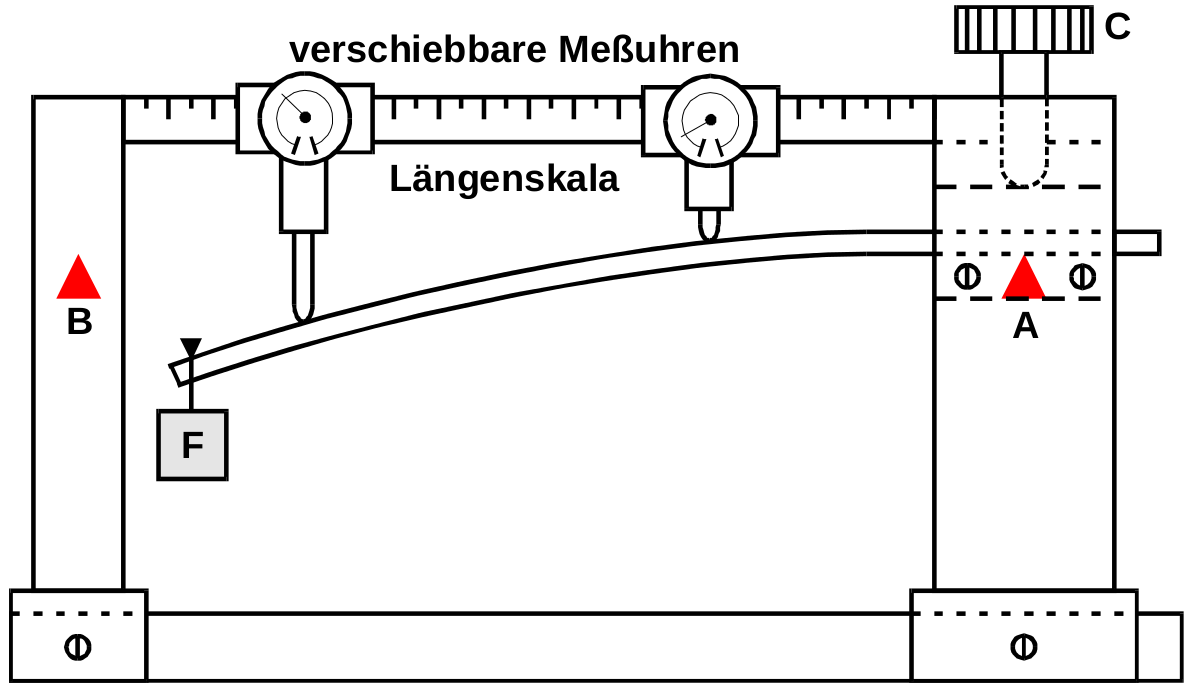
\includegraphics[scale=0.2]{content/aufbau.png}
    \caption{Schematischer Aufbau der Apperatur [1]}
    \label{fig:abb2}
\end{figure}

Mit dieser Apperatur werden beide Messungen durchgeführt. Zunächst wird
der Stab einseitig eingespannt. Mit Hilfe der verschiebbaren Messuhren 
wird eine Messung der Durchbiegung des Stabes ohne angehängtes Gewicht 
vorgenommen. Anschließend wird die Messung mit einem angehängtem 
Gewicht wiederholt, um aus der Differenz die tatsächliche Durchbiegung
bestimmen zu können. Zudem wird die Länge $L$ zwischen Gewicht und 
Einspannung bestimmt. Diese Messung wird jeweils mit einem eckigen und 
einem runden Stab durchgeführt und das angehängte Gewicht $m_1$ gewogen.
\\
Bei der zweiten Messung wird der Stab beidseitig an den Punkten A und B 
aufgelegt. Wieder wird erst eine Messung ohne Gewicht durchgeführt, 
bevor dieses in der Mitte des Stabes eingehängt wird. Diese 
Messung wird nur für einen rechteckigen Stab durchgeführt. Wieder 
wird die Masse $m_2$ des angehängten Gewichtes bestimmt. 
\\
Zuletzt werden die verwendeten Stäbe vermessen. 
